\chapter{Finite element assembly}
\label{sec:assembly}

\newtheorem{example}{\small{\sc{Example}}}[section]

In this section, we present a general algorithm for assembly of finite
element variational forms and define the concepts that the UFC
interface is based on.

\section{Finite Element Discretization}
\label{sec:fem}

\subsection{The Finite Element}
\index{finite element}

A finite element is mathematically defined as a triplet consisting of
a polygon, a polynomial function space, and a set of linear
functionals, see~\cite{Cia78}. Given that the dimension of the
function space and the number of the (linearly independent) linear
functionals are equal, the finite element is uniquely defined. Hence,
we will refer to a finite element as a collection of
\begin{itemize}
\item a polygon $K$,
\item a polynomial space $\mathcal{P}_K$ on $K$,
\item a set of linearly independent linear functionals, the
\emph{degrees of freedom}, $L_i : \mathcal{P}_K \rightarrow \R, \, i =
1, 2, \ldots, n$.
\end{itemize}

\subsection{Variational Forms}
\index{variational form}

Consider the weighted Poisson problem $- \nabla \cdot (w \nabla u) =
f$ with Dirichlet boundary conditions on a domain $\Omega \subset
\R^d$.  Multiplying by a test function $v \in V_h$ and integrating by
parts, one obtains the variational problem
\begin{equation} \label{eq:weightedpoisson}
  \int_{\Omega} w \nabla v \cdot \nabla u \dx = \int_{\Omega} v f \dx
  \quad \forall v \in V_h,
\end{equation}
for $u \in V_h$. If $w, f \in W_h$ for some discrete finite element space
$W_h$ (which may be different from $V_h$), we may thus
write~(\ref{eq:weightedpoisson}) as
\begin{equation}
  a(v, u; w) = L(v; f) \quad \forall v \in V_h,
\end{equation}
where the trilinear form $a : V_h \times V_h \times W_h \rightarrow \R$ is given by
\begin{equation}
  a(v, u; w) = \int_{\Omega} w \nabla v \cdot \nabla u \dx
\end{equation}
and the bilinear form $L : V_h \times W_h \rightarrow R$ is given by
\begin{equation}
  L(v; f) = \int_{\Omega} v f \dx.
\end{equation}
Note here that $a$ is \emph{bilinear} for any given fixed $w \in W_h$
and $L$ is \emph{linear} for any given fixed $f \in W_h$.

In general, we shall be concerned with the discretization of
finite element variational forms of general arity~$r + n > 0$,
\begin{equation} \label{eq:variationalform}
  a : V_h^1 \times V_h^2 \times \cdots \times V_h^r \times
  W_h^1 \times W_h^2 \times \cdots \times W_h^n \rightarrow \R,
\end{equation}
defined on the product space $V_h^1 \times V_h^2 \times \cdots \times
V_h^r \times W_h^1 \times W_h^2 \times \cdots \times W_h^n$ of two
sets $\{V_h^j\}_{j=1}^r, \{W_h^j\}_{j=1}^n$ of discrete finite element
function spaces on $\Omega$. We refer to
$(v_1, v_2, \ldots, v_r) \in V_h^1 \times V_h^2 \times \cdots \times V_h^r$
as \emph{primary arguments},
and to
$(w_1, w_2, \ldots, w_n) \in W_h^1 \times W_h^2 \times \cdots \times W_h^n$
as \emph{coefficients} and write
\begin{equation}
a = a(v_1, \ldots, v_r; w_1, \ldots, w_n).
\label{eq:gen_form}
\end{equation}
In the simplest case, all function spaces are equal but there are many
important examples, such as mixed methods, where the
arguments come from different function spaces.

\subsection{Discretization}
\label{sec:Discretization}

To discretize the form $a$, we introduce bases
$\{\phi_i^1\}_{i=1}^{N^1},
 \{\phi_i^2\}_{i=1}^{N^2}, \ldots,
 \{\phi_i^r\}_{i=1}^{N^r}$
for the function spaces $V_h^1, V_h^2, \ldots, V_h^r$ respectively and let $i =
(i_1, i_2, \ldots, i_r)$ be a multiindex of length $|i| = r$. The
form $a$ then defines a rank~$r$ tensor given by
\begin{equation} \label{eq:tensor}
  A_i = a(\phi_{i_1}^1, \phi_{i_2}^2, \ldots, \phi_{i_r}^r; w_1, w_2, \ldots, w_n)
  \quad \forall i \in \mathcal{I},
\end{equation}
where $\mathcal{I}$ is the index set
\begin{equation}
  \begin{split}
  & \mathcal{I} =  \prod_{j=1}^r[1,|V^j_h|] =  \\
  & \{(1,1,\ldots,1), (1,1,\ldots,2), \ldots,
  (N^1,N^2,\ldots,N^r)\}.
  \end{split}
\end{equation}
We refer to the tensor~$A$ as the \emph{discrete operator} generated
by the form~$a$ and the particular choice of basis functions.  For any
given form of arity~$r + n$, the tensor~$A$ is a (typically sparse)
tensor of rank~$r$ and dimension $|V_h^1| \times |V_h^2| \times \ldots
\times |V_h^r| = N^1 \times N^2 \times \ldots \times N^r$.
\index{global tensor}

Typically, the rank $r$ is 0, 1, or 2. When $r = 0$, the
tensor $A$ is a scalar (a tensor of rank zero), when $r = 1$, the
tensor $A$ is a vector (the ``load vector'') and when $r = 2$, the
tensor $A$ is a matrix (the ``stiffness matrix''). Forms of higher
arity also appear, though they are rarely assembled as a
higher-dimensional sparse tensor.

Note here that we consider the functions $w_1, w_2, \ldots, w_n$ as
fixed in the sense that the discrete operator~$A$ is computed for a
given set of functions, which we refer to as \emph{coefficients}. As
an example, consider again the variational
problem~(\ref{eq:weightedpoisson}) for the weighted Poisson's
equation. For the trilinear form~$a$, the rank is $r = 2$ and
the number of coefficients is $n = 1$, while for the linear form~$L$,
the rank is $r = 1$ and the number of coefficients is $n = 1$. We may
also choose to directly compute the \emph{action} of the form
$a$ obtained by assembling a vector from the form
\begin{equation}
  a(v_1; w_1, w2) = \int_{\Omega} w_1 \nabla v_1 \cdot \nabla w_2 \dx,
\end{equation}
where now $r = 1$ and $n = 2$.

We list below a few other examples to illustrate the notation.

\begin{example}
\label{example:div}
Our first example is related
to the divergence constraint in fluid flow. Let the form~$a$ be given by
\begin{equation}
a(q, u) = \int_{\Omega} q \nabla \cdot u \dx, \quad q\in V_h^1, \quad u\in V_h^2, 
\end{equation}
where $V_h^1$ is a space of scalar-valued functions and where $V_h^2$
is a space of vector-valued functions.  The form $a : V_h^1 \times
V_h^2 \rightarrow \R$ has two primary arguments and thus $r = 2$.
Furthermore, the form does not depend on any coefficients and thus $n=0$.
\end{example}

\begin{example}
\label{example:linearconv}
Another common form in fluid flow (with variable density) is
\begin{equation}
a(v,u;w,\varrho) = \int_{\Omega} v \, \varrho \, w \cdot \nabla  u \dx. 
\end{equation}
Here, $v\in V_h^1,\ u \in V_h^2,\ w\in W_h^1, \ \varrho \in W_h^2$, where
$V_h^1$, $V_h^2$, and $W_h^1$ are spaces of vector-valued functions, while $W_h^2$ is a space of  
scalar-valued functions. 
The form takes four arguments, where two of the arguments
are coefficients,
\begin{equation}
a : V_h^1 \times V_h^2 \times W_h^1 \times W_h^2 \rightarrow \R.
\end{equation}
Hence, $r=2$ and $n=2$. 
\end{example}

\begin{example}
The $H^1(\Omega)$ norm of the error $e = u - u_h$ squared is
\begin{equation}
a(;u, u_h) = \int_{\Omega} (u - u_h)^2 + |\nabla (u - u_h)|^2 \dx.
\end{equation}
The form takes two arguments and both are coefficients,
\begin{equation}
a : W_h^1 \times  W_h^2 \rightarrow \R.
\end{equation}
Hence, $r=0$ and $n=2$. 
\end{example}

\section{Finite Element Assembly}
\index{assembly}

The standard algorithm for computing the global sparse tensor~$A$ is
known as \emph{assembly}, see~\cite{ZieTay67,Hug87}. By this
algorithm, the tensor~$A$ may be computed by assembling (summing) the
contributions from the local entities of a finite element mesh.  To
express this algorithm for assembly of the global sparse tensor~$A$ for
a general finite element variational form of arity~$r$, we introduce
the following notation and assumptions.

Let $\mathcal{T} = \{K\}$ be a set of disjoint \emph{cells} (a
triangulation) partitioning the domain $\Omega =
\cup_{K\in\mathcal{T}} K$. Further, let $\partial_e \mathcal{T}$
denote the set of \emph{exterior facets} (the set of cell facets
incident with the boundary $\partial \Omega$), and let $\partial_i
\mathcal{T}$ denote the set of $\emph{interior facets}$ (the set of
cell facets non-incident with the boundary $\partial \Omega$).  For
each discrete function space $V_h^j, \, j=1,2,\ldots,r$, we assume
that the global basis~$\{\phi_i^j\}_{i=1}^{N^j}$ is obtained by
patching together local function spaces $\mathcal{P}_K^j$ on each
cell~$K$ as determined by a local-to-global mapping.

We shall further assume that the variational
form~(\ref{eq:variationalform}) may be expressed as a sum of integrals
over the cells~$\mathcal{T}$, the exterior facets~$\partial_e
\mathcal{T}$ and the interior facets~$\partial_i \mathcal{T}$. We
shall allow integrals expressed on disjoint subsets
$\mathcal{T} = \cup_{k=1}^{n_c} \mathcal{T}_k$,
$\partial_e \mathcal{T} = \cup_{k=1}^{n_e} \partial_e \mathcal{T}_k$
and
$\partial_i \mathcal{T} = \cup_{k=1}^{n_i} \partial_i \mathcal{T}_k$
respectively.

We thus assume that the form $a$ is given by
\begin{equation}
  \begin{split}
    & a(v_1, \ldots, v_r; w_1, \ldots,  w_n) =  \\
    &\ \ \   \sum_{k=1}^{n_c} \sum_{K\in\mathcal{T}_k} \int_{K}
    I^c_k(v_1, \ldots, v_r; w_1, \ldots w_n) \dx \\
    &+
    \sum_{k=1}^{n_e} \sum_{S\in\partial_e\mathcal{T}_k} \int_{S}
    I^e_k(v_1, \ldots, v_r; w_1, \ldots,  w_n) \ds \\
    &+
    \sum_{k=1}^{n_i} \sum_{S\in\partial_i\mathcal{T}_k} \int_{S}
    I^i_k(v_1, \ldots, v_r; w_1, \ldots, w_n) \ds.
  \end{split} \label{eq:form_integrals}
\end{equation}
We refer to an integral over a cell~$K$ as a \emph{cell integral},
an integral over an exterior facet~$S$ as an \emph{exterior facet integral}
(typically used to implement Neumann and Robin type boundary conditions),
and to an integral over an interior facet~$S$ as an \emph{interior facet integral} (typically used in discontinuous Galerkin methods).

For simplicity, we consider here initially assembly of the global
sparse tensor~$A$ corresponding to a form~$a$ given by a single
integral over all cells $\mathcal{T}$, and later extend to the general
case where we must also account for contributions from several cell
integrals, interior facet integrals and exterior facet integrals.

We thus consider the form
\begin{equation}
  \begin{split}
    &a(v_1, \ldots, v_r; w_1, \ldots, w_n) = \\
    & \ \ \ \sum_{K\in\mathcal{T}} \int_K
    I^c(v_1, \ldots, v_r; w_1, \ldots, w_n) \dx,
  \end{split}
\end{equation}
for which the global sparse tensor~$A$ is given by
\begin{equation}
  A_i = \sum_{K\in\mathcal{T}} \int_K
  I^c(\phi^1_{i_1}, \ldots, \phi^r_{i_r}; w_1, \ldots, w_n) \dx.
\end{equation}
To see how to compute the tensor $A$ by summing the local
contributions from each cell~$K$, we let $n^j_K = |\mathcal{P}^j_K|$
denote the dimension of the local finite element space on $K$ for the
$j$th primary argument $v_j \in V_h^j$ for $j = 1,2,\ldots,r$. Furthermore, let
\begin{equation}
  \iota_K^j : [1,n_K^j] \rightarrow [1,N^j] \label{eq:iota_K}
\end{equation}
denote the local-to-global mapping for~$V_h^j$, that is, on any given
$K\in\mathcal{T}$, the mapping $\iota_K^j$ maps the number of a local
degree of freedom (or, equivalently, local basis function) to the
number of the corresponding global degree of freedom (or,
equivalently, global basis function). We then define for each $K \in
\mathcal{T}$ the collective local-to-global mapping $\iota_K :
\mathcal{I}_K \rightarrow \mathcal{I}$ by
\begin{equation}
  \iota_K(i) =
  (\iota_K^1(i_1),\iota_K^2(i_2),\ldots,\iota_K^r(i_r))
  \quad \forall i \in \mathcal{I}_K,
\end{equation}
where $\mathcal{I}_K$ is the index set
\begin{equation}
\begin{split}
  & \mathcal{I}_K = \prod_{j=1}^r[1,|\mathcal{P}_K^j|] \\ 
  & = \{(1,1,\ldots,1), (1,1,\ldots,2), \ldots,
  (n_K^1,n_K^2,\ldots,n_K^r)\}.
\end{split}
\end{equation}
Furthermore, for each $V_h^j$ we let $\{\phi^{K,j}_i\}_{i=1}^{n_K^j}$
denote the restriction to an element $K$ of the subset of the basis
$\{\phi_i^j\}_{i=1}^{N^j} \subset \mathcal{P}_K^j$ of $V_h^j$ supported on $K$.

We may now compute~$A$ by summing the contributions from
the local cells,
\begin{equation}
  \begin{split}
  A_i
  &=
  \sum_{K\in\mathcal{T}_i} \int_K
  I^c(\phi_{i_1}^1, \ldots, \phi_{i_r}^r; w_1, \ldots, w_n) \dx \\
  &=
  \sum_{K\in\mathcal{T}_i} \int_K
  I^c(\phi_{(\iota_K^1)^{-1}(i_1)}^{K,1},
      \ldots,
      \phi_{(\iota_K^r)^{-1}(i_r)}^{K,r}; w_1, \ldots, w_n) \dx \\
  &=
  \sum_{K\in\mathcal{T}_i}
  A^K_{\iota_K^{-1}(i)},
  \end{split}
\end{equation}
where $A^K$ is the local \emph{cell tensor} on cell $K$ (the ``element
stiffness matrix''), given by
\begin{equation}
  A^K_i = \int_K
  I^c(\phi_{i_1}^{K,1},
  \ldots,
  \phi_{i_r}^{K,r}; w_1, \ldots, w_n) \dx, \\
\end{equation}
and where $\mathcal{T}_i$ denotes the set of cells on which all basis
functions $\phi_{i_1}^1, \phi_{i_2}^2, \ldots, \phi_{i_r}^r$ are supported.
Similarly, we may sum the local contributions
from the exterior and interior facets in the form of local
\emph{exterior facet tensors} and \emph{interior facet tensors}.
\index{cell tensor}
\index{exterior facet tensor}
\index{interior facet tensor}

\begin{figure}[htbp]
  \begin{center}
    \psfrag{i0}{\hspace{-0.5cm}$\iota_K^1(1)$}
    \psfrag{i1}{\hspace{-0.5cm}$\iota_K^1(2)$}
    \psfrag{i2}{\hspace{-0.5cm}$\iota_K^1(3)$}
    \psfrag{j0}{\hspace{-0.3cm}$\iota_K^2(1)$}
    \psfrag{j1}{\hspace{-0.5cm}$\iota_K^2(2)$}
    \psfrag{j2}{\hspace{-0.1cm}$\iota_K^2(3)$}
    \psfrag{A21}{$A^K_{32}$}
    \psfrag{1}{$1$}
    \psfrag{2}{$2$}
    \psfrag{3}{$3$}
    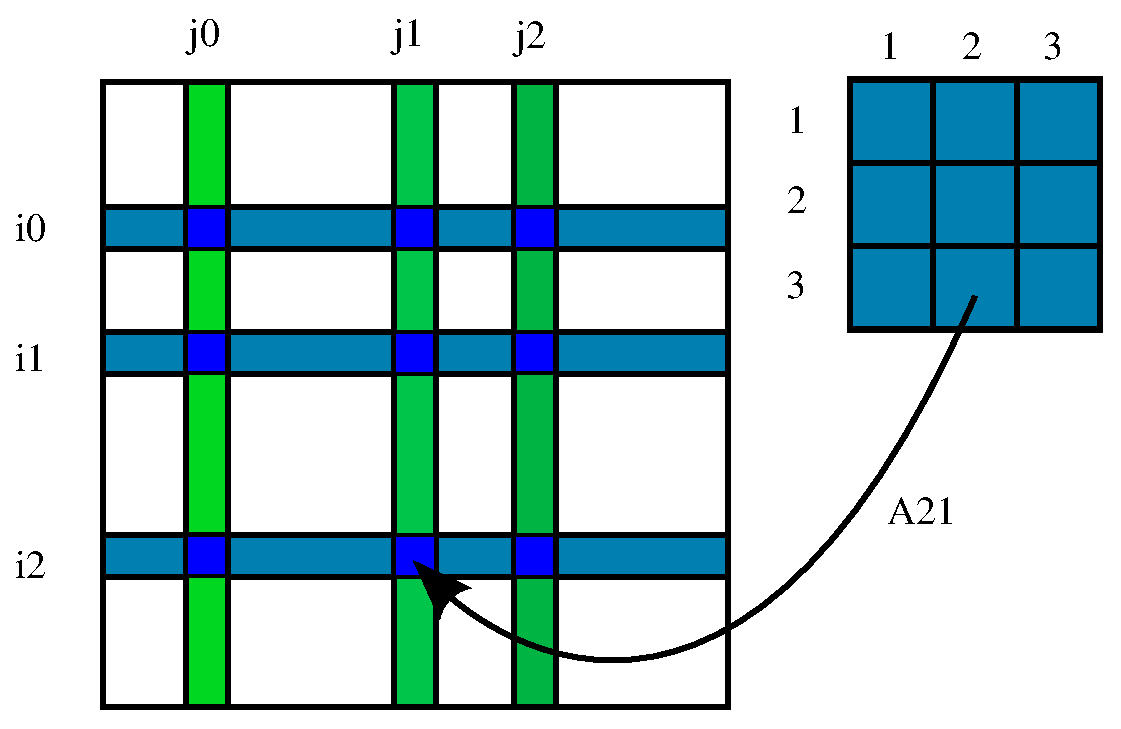
\includegraphics[height=3in]{eps/insertion.eps}
    \caption{Adding the entries of a cell tensor~$A^K$ to the
      global tensor~$A$ using the  local-to-global mapping
      $\iota_K$, illustrated here for a rank two
      tensor (a matrix).}
    \label{fig:insertion}
  \end{center}
\end{figure}

In Algorithm~\ref{alg:assembly}, we present a general algorithm for
assembling the contributions from the local cell, exterior facet and
interior facet tensors into a global sparse tensor.  In all cases, we
iterate over all entities (cells, exterior or interior facets),
compute the local cell tensor $A^K$ (or exterior/interior facet tensor
$A^S$) and add it to the global sparse tensor as determined by the
local-to-global mapping, see~Figure~\ref{fig:insertion}.


\begin{algorithm}
\footnotesize
$A = 0$ \\
(i) \emph{Assemble contributions from all cells} \\
\textbf{for each} $K \in \mathcal{T}$ \\
\\
\tab \textbf{for} $j = 1,2,\ldots,r$: \\
\tab\tab Tabulate the local-to-global mapping $\iota_K^j$ \\
\\
\tab \textbf{for} $j = 1,2,\ldots,n$: \\
\tab\tab Extract the values of $w_j$ on $K$
\\
\\
\tab Take $0 \leq k \leq n_c$ such that $K \in \mathcal{T}_k$ \\
\tab Tabulate the cell tensor $A^K$ for $I^c_k$ \\
\tab Add $A^K_i$ to $A_{\iota_K^1(i_1), \iota_K^2(i_2), \ldots, \iota_K^r(i_r)}$ for $i\in I_K$ \\
\\
(ii) \emph{Assemble contributions from all exterior facets} \\
\textbf{for each} $S \in \partial_e\mathcal{T}$ \\
\\
\tab \textbf{for} $j = 1,2,\ldots,r$: \\
\tab\tab Tabulate the local-to-global mapping $\iota_{K(S)}^j$ \\
\\
\tab \textbf{for} $j = 1,2,\ldots,n$: \\
\tab\tab Extract the values of $w_j$ on $K(S)$
\\
\\
\tab Take $0 \leq k \leq n_e$ such that $S \in \partial_e \mathcal{T}_k$ \\
\tab Tabulate the exterior facet tensor $A^S$ for $I^e_k$ \\
\tab Add $A^S_i$ to $A_{\iota_{K(S)}^1(i_1), \iota_{K(S)}^2(i_2), \ldots, \iota_{K(S)}^r(i_r)}$ for $i\in I_{K(S)}$ \\
\\
\\
(iii) \emph{Assemble contributions from all interior facets} \\
\textbf{for each} $S \in \partial_i\mathcal{T}$ \\
\\
\tab \textbf{for} $j = 1,2,\ldots,r$: \\
\tab\tab Tabulate the local-to-global mapping $\iota_{K(S)}^j$ \\
\\
\tab \textbf{for} $j = 1,2,\ldots,n$: \\
\tab\tab Extract the values of $w_j$ on $K(S)$
\\
\\
\tab Take $0 \leq k \leq n_i$ such that $S \in \partial_i \mathcal{T}_k$ \\
\tab Tabulate the interior facet tensor $A^S$ for $I^i_k$ \\
\tab Add $A^S_i$ to $A_{\iota_{K(S)}^1(i_1), \iota_{K(S)}^2(i_2), \ldots, \iota_{K(S)}^r(i_r)}$ for $i\in I_{K(S)}$ \\
\caption{Assembling the global tensor~$A$ from the local contributions
  on all cells, exterior and interior facets. For assembly over
  exterior facets, $K(S)$ refers to the cell $K\in\mathcal{T}$ incident
  to the exterior facet~$S$, and for assembly over interior facets,
  $K(S)$ refers to the ``macro cell'' consisting of the pair of cells
  $K^+$ and $K^-$ incident to the interior facet~$S$.}
\label{alg:assembly}
\end{algorithm}
\normalsize
